\chapter{Fazit und Ausblick}
\section{Fazit}
In dieser Arbeit wurde der 32-Bit Softcore Prozessor Microblaze von Xilinx in die SpartanMC Entwicklungsumgebung integriert. Anhand der Abbildung \ref{fig:Schaubild} wird beschrieben, welche Schritte dafür erforderlich waren und zu welchem Grad der Microblaze integriert werden konnte.\\
Zu Beginn musste der Prozessor zusammen mit einem Speichermodul, einem FSL-Modul und einem UART-Core in den Systembuilder JConfig integriert werden. Hierzu wurden für die neue Hardware XML-Modulbeschreibungen erstellt, welche sämtliche Parameter und Signale der Komponenten definieren. Desweiteren wurden Wrapper-Module in Verilog und VHDL erstellt und der SpartanMC Hardware-Library hinzugefügt. Diese Wrapper instanziieren die neuen Cores mit den über JConfig getroffenen Einstellungen. Außerdem wurde ein neuer, generischer Speicher für den Microblaze in Verilog geschrieben, da kein generisches Modell vorhanden war. JConfig wurde dahingehend angepasst, dass es eine neue Memory-Map in Form einer BMM-Datei erzeugt, sobald ein Microblaze im System vorhanden ist. Das Xilinx Tool data2mem, welches zur Initialisierung und Aktualisierung von Block RAMs verwendet wird, wurde in die Toolchain integriert, um die Speicherinitialisierung für den Microblaze zu realisieren. Dieses Tool erlaubt es UCF-Dateien zu erzeugen, die in der Synthese dafür sorgen, dass die Speicher korrekt initialisiert werden. Außerdem ist data2mem in der Lage existierende Bitfiles zu aktualisieren ohne die Synthese erneut zu starten und es ist außerdem in der Lage Speicherinitialisierungen für die Simulation in Form von Verilog-Dateien zu erzeugen. Desweitern wurde im Rahmen dieser Arbeit das Konzept von Simulationslibraries in die Toolchain integriert. Dies erlaubt es VHDL-Dateien in Libraries zusammenzufassen und diese vorzukompilieren, sodass sie während der Simulation nicht erneut kompiliert werden müssen.\\
\section{Ausblick}
Im Rahmen dieser Arbeit konnte aus zeitliche Gründen allerdings nicht mehr die Integration des Microblaze GCC in die Toolchain realisiert werden. So ist die Toolchain nicht in der Lage, für den Microblaze kompatible ELF-Dateien zu erzeugen und muss daher auf extern erzeugte Varianten zurückgreifen. Desweiteren konnte keine erfolgreiche Datenübertragung über das AXI-Interface des Microblaze umgesetzt werden. In zukünftigen Arbeiten sollten daher zunächst diese beiden Probleme behoben werden. Neben diesen Punkten gibt es eine Reihe weiterer Möglichkeiten, diese Arbeit fortzusetzen. Es sollte auf jeden Fall der IP-Core für den AXI4-Bus in JConfig integriert werden, um es zu ermöglichen mehr als nur eine Peripherie an den Microblaze anzuschließen. Desweiteren wurde das optionale Ziel dieser Arbeit, die Paralellisierung eines Microblaze Programms mit \textmu\/Streams, nicht erfüllt. Hierzu wäre es notwendig, \textmu\/Streams dahingehend anzupassen, dass eine entsprechende Hardwarekonfiguration mit den neu integrierten Komponenten erstellt werden kann und die Aufrufe der Core-Konnektoren durch Aufrufe der FSL-Blöcke ersetzt werden. Außerdem wäre es interessant die verschiedenen Konfigurationsmöglichkeiten (z.b. externer Speicher mit Caches, MMU, Debug-Modul, ...) des Microblaze auszuprobieren, da im Rahmen dieser Arbeit nur die Standardkonfiguration getestet wurde. Eine Möglichkeit die Nutzbarkeit von Simulationlibraries zu verbessern, wäre es, die kompletten Bibliotheken zu erzeugen und an einem, im Fachbereich Rechnersysteme global zugänglichem Verzeichnis abzulegen. Dies ist unter Berücksichtigung der Möglichkeit, dass weitere IP-Cores von Xilinx in Zukunft integriert werden und der langen Kompilierungszeit der Libraries durchaus sinnvoll.
\begin{figure}
\centering
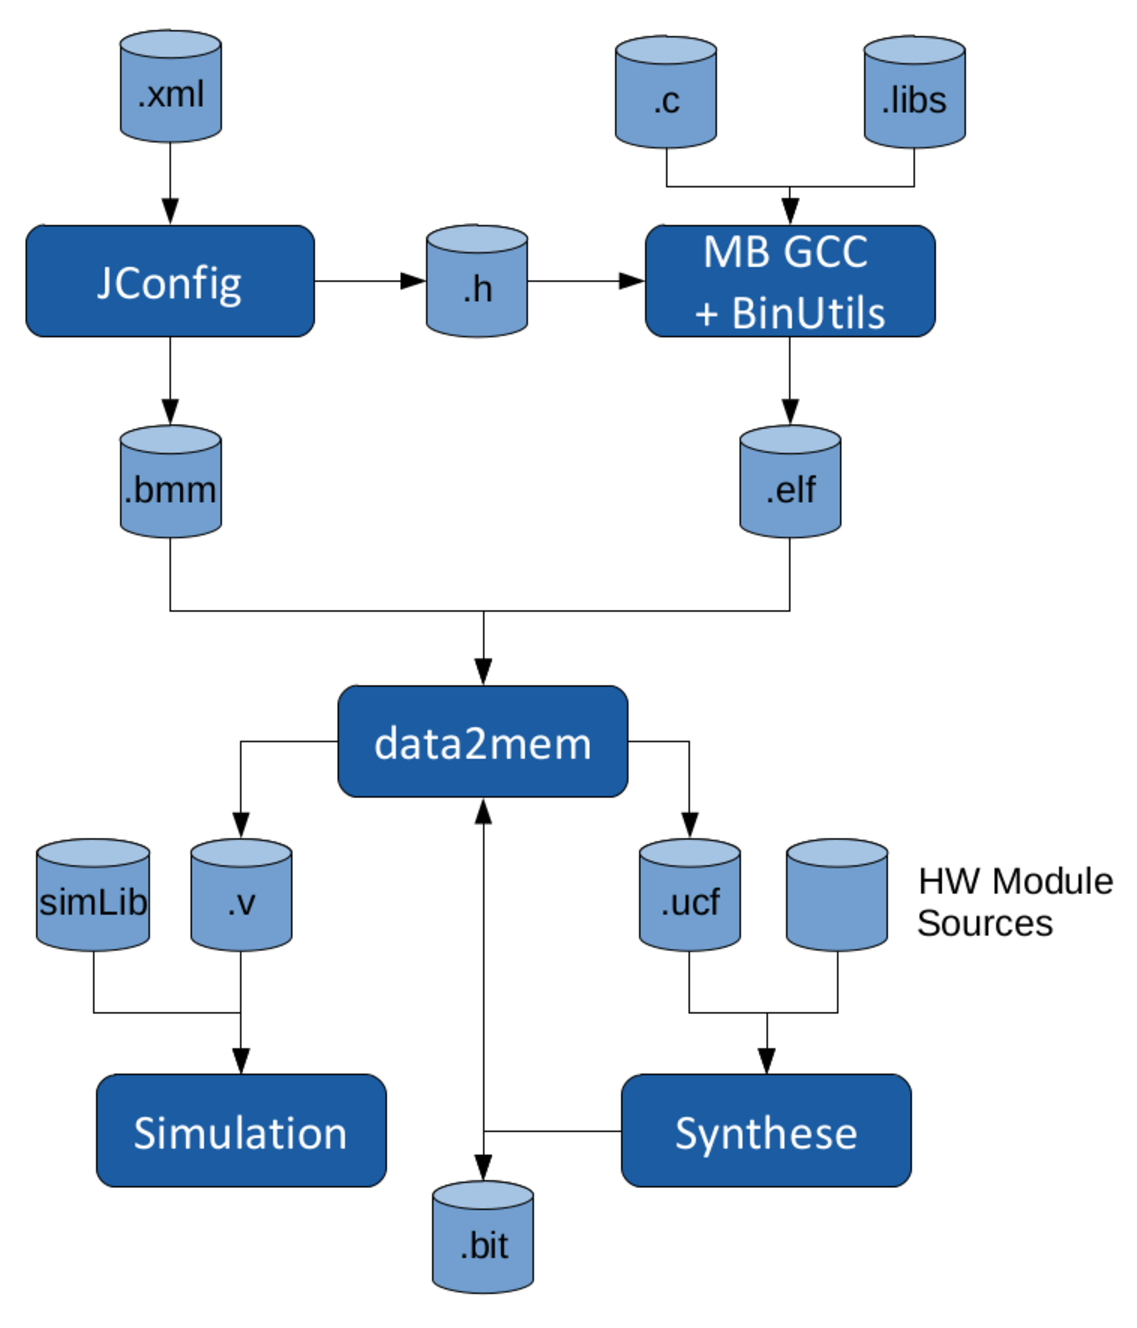
\includegraphics[width=0.8\linewidth, height=0.8\linewidth]{./bilder/Schaubild}
\caption{Schaubild zu den Neuerungen die im Rahmen dieser Arbeit vorgenommen wurden}
\label{fig:Schaubild}
\end{figure}